\subsection{Itération n°1}

\subsubsection{Configuration et modifications}

Nous décidons de ne plus utiliser de \emph{squashed gaussian} dans l'évaluation de l'acteur. Cela nous permet de voir plus finement le comportement de la distribution normal que cache la fonction tangente hyperbolique. A la place, nous choisissons de calculer l'action à partir une distribution normale dont l'écart-type est imposé à $1,5$ pour qu'il y ait de l'exploration en tout temps.

Nous décidons de ne plus calculer le gradient par sommation des récompenses pour réduire le temps de calcul.

\subsubsection{Analyse}

\begin{figure}[H]
    \centering
    \begin{subfigure}{0.3\textwidth}
        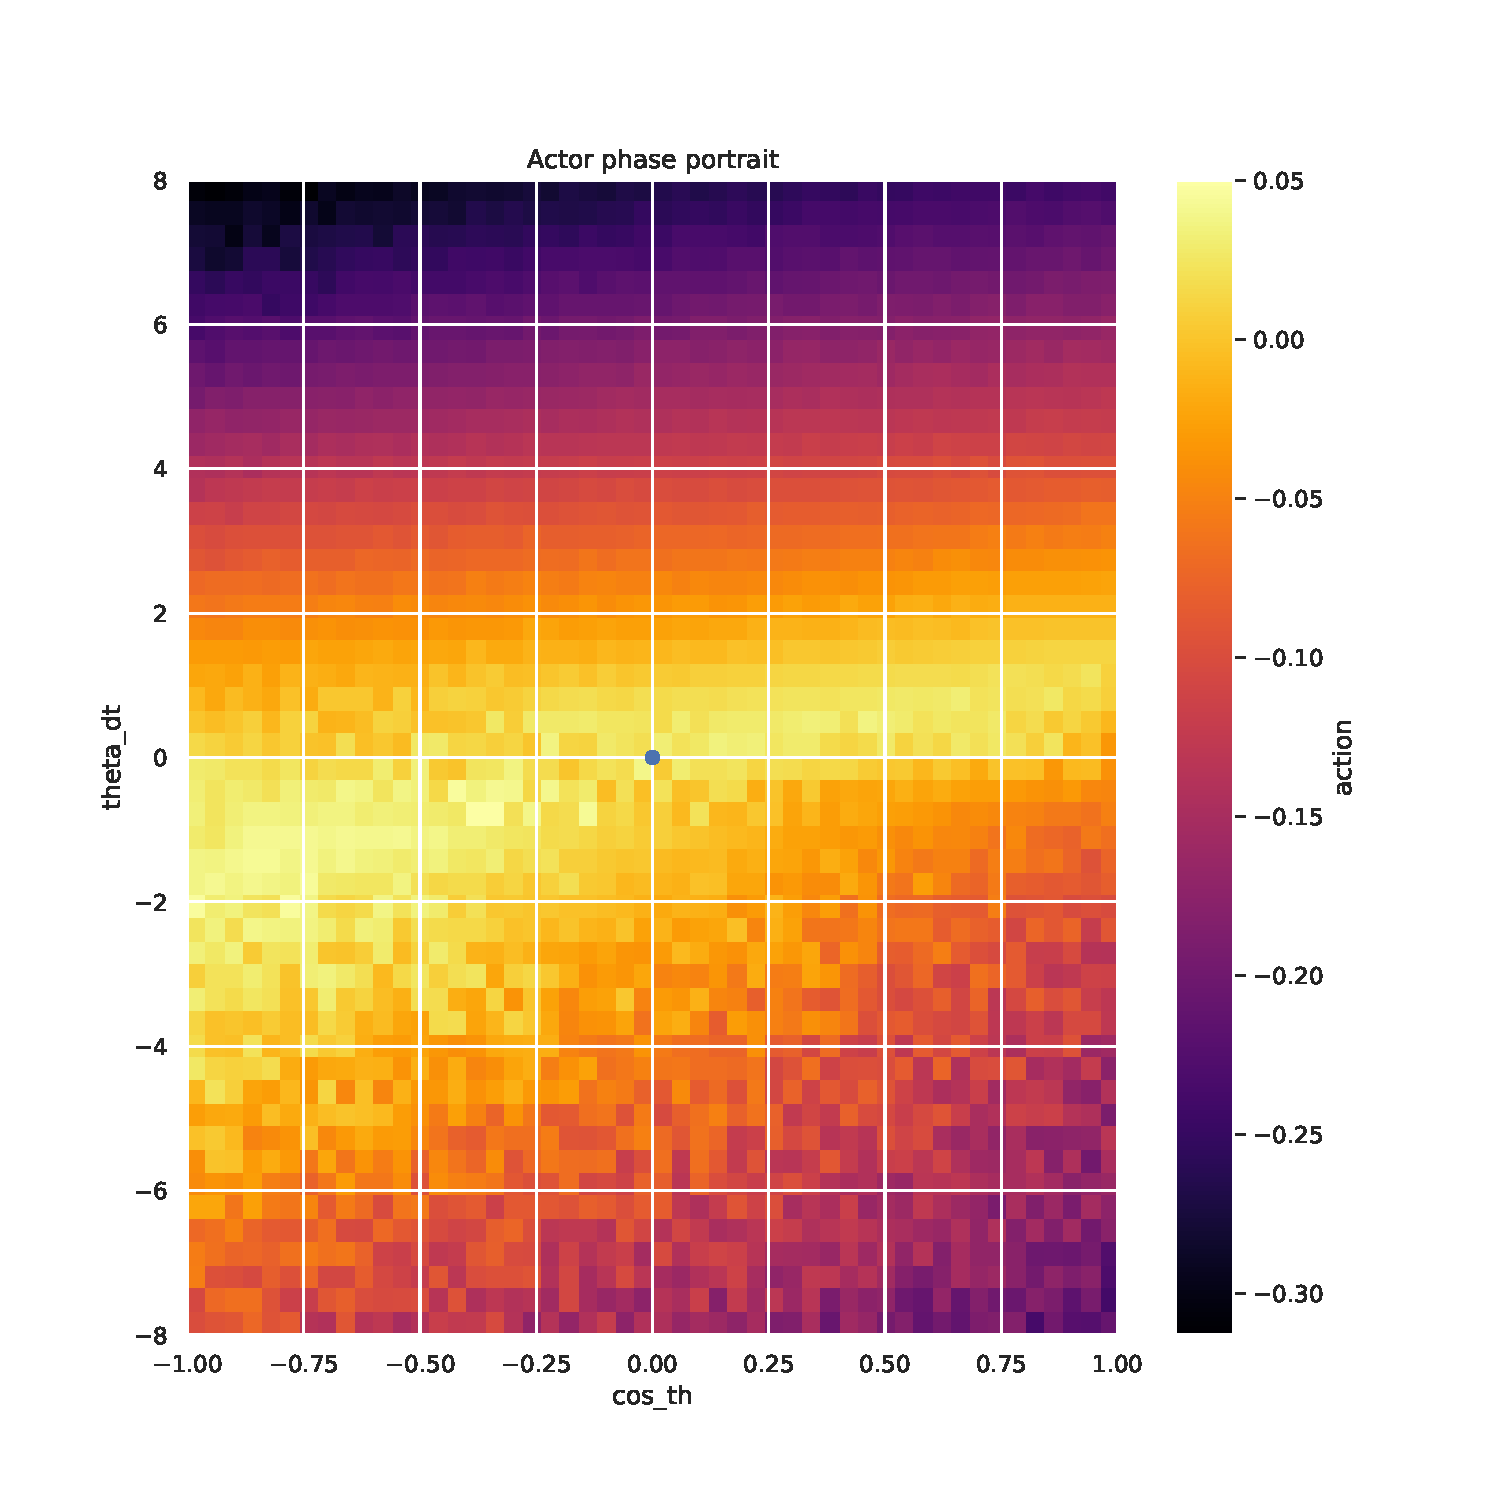
\includegraphics[width=\textwidth]{figures/iteration1/0_actor_discount__ante_Pendulum-v0.pdf}
        \caption{Acteur naïf}
    \end{subfigure}
    \begin{subfigure}{0.3\textwidth}
        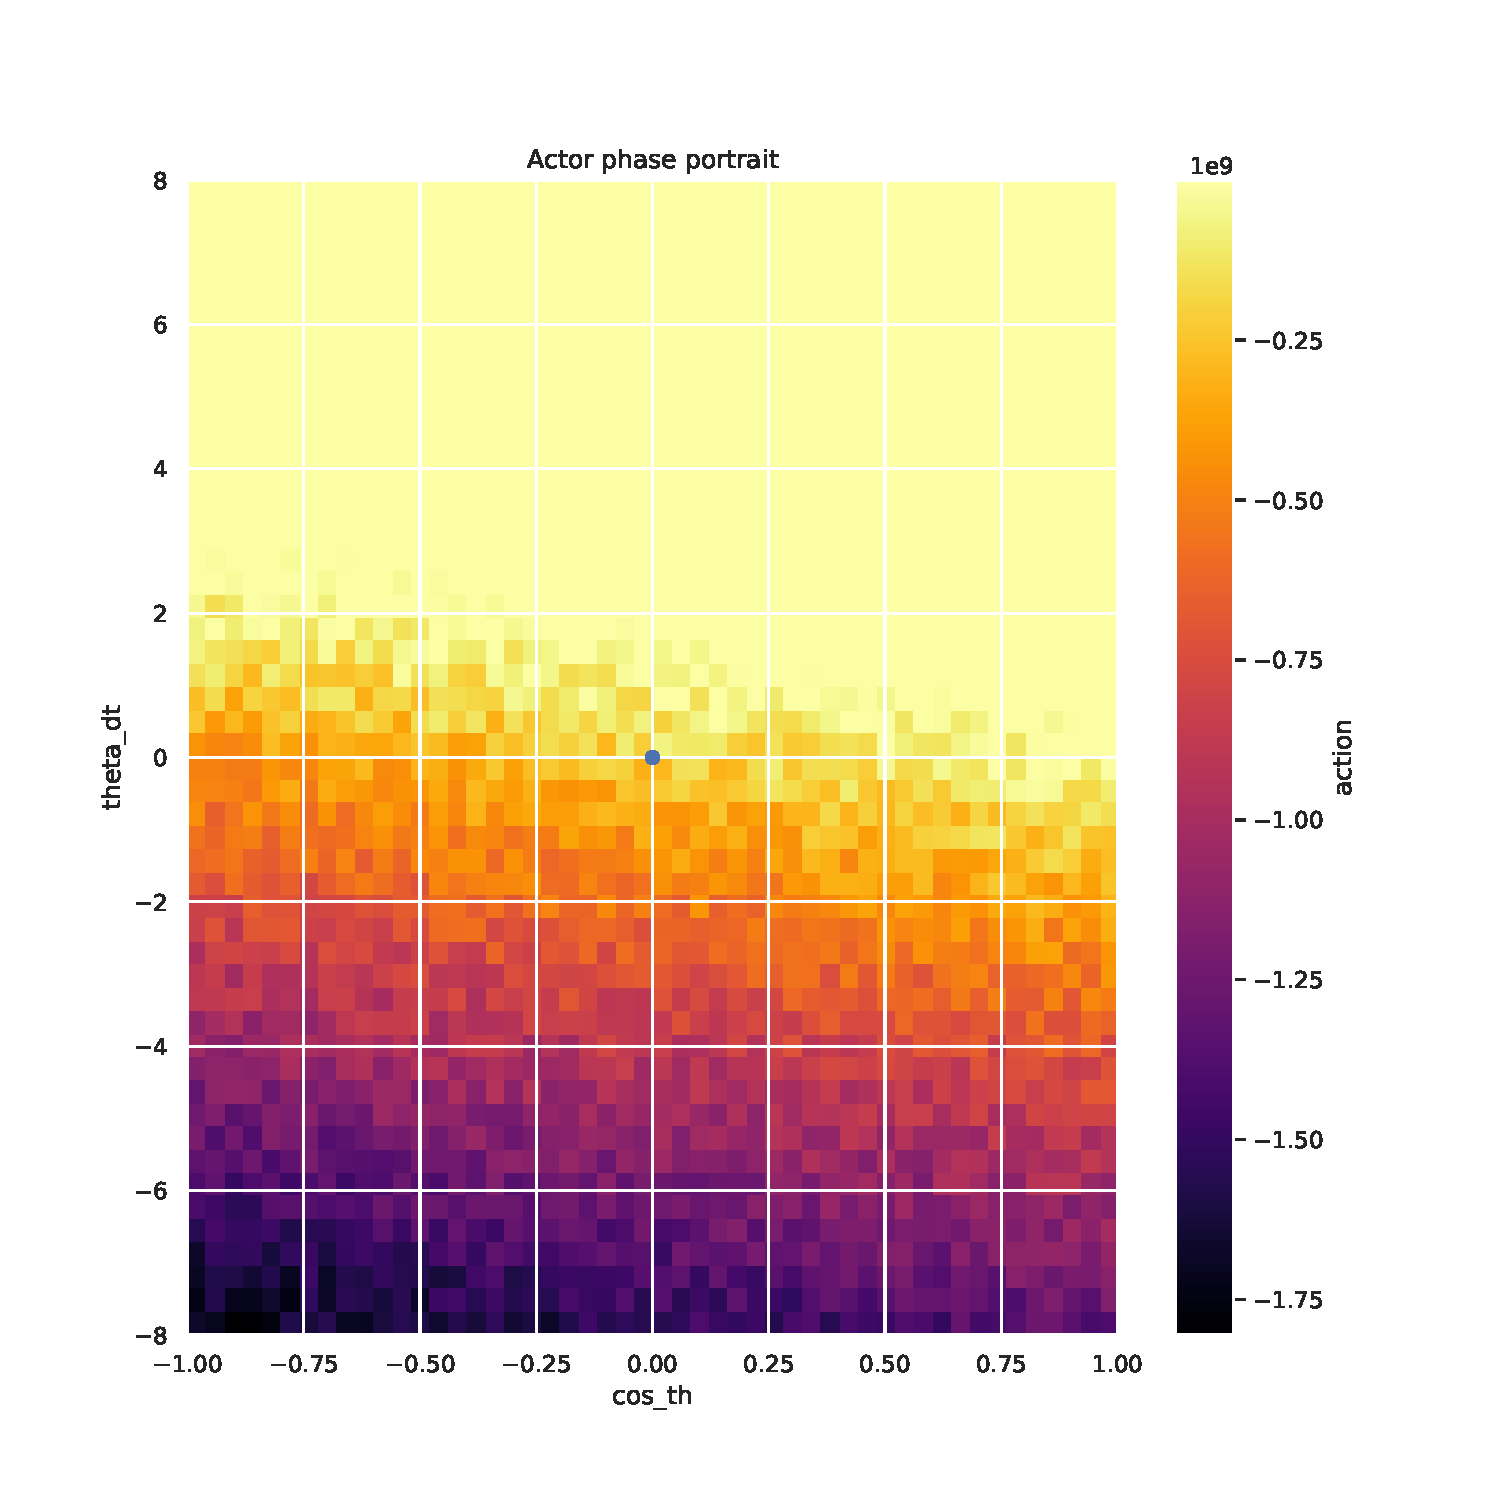
\includegraphics[width=\textwidth]{figures/iteration1/0_actor_discount__post_Pendulum-v0.pdf}
        \caption{Acteur entraîné}
    \end{subfigure}
    \begin{subfigure}{0.3\textwidth}
        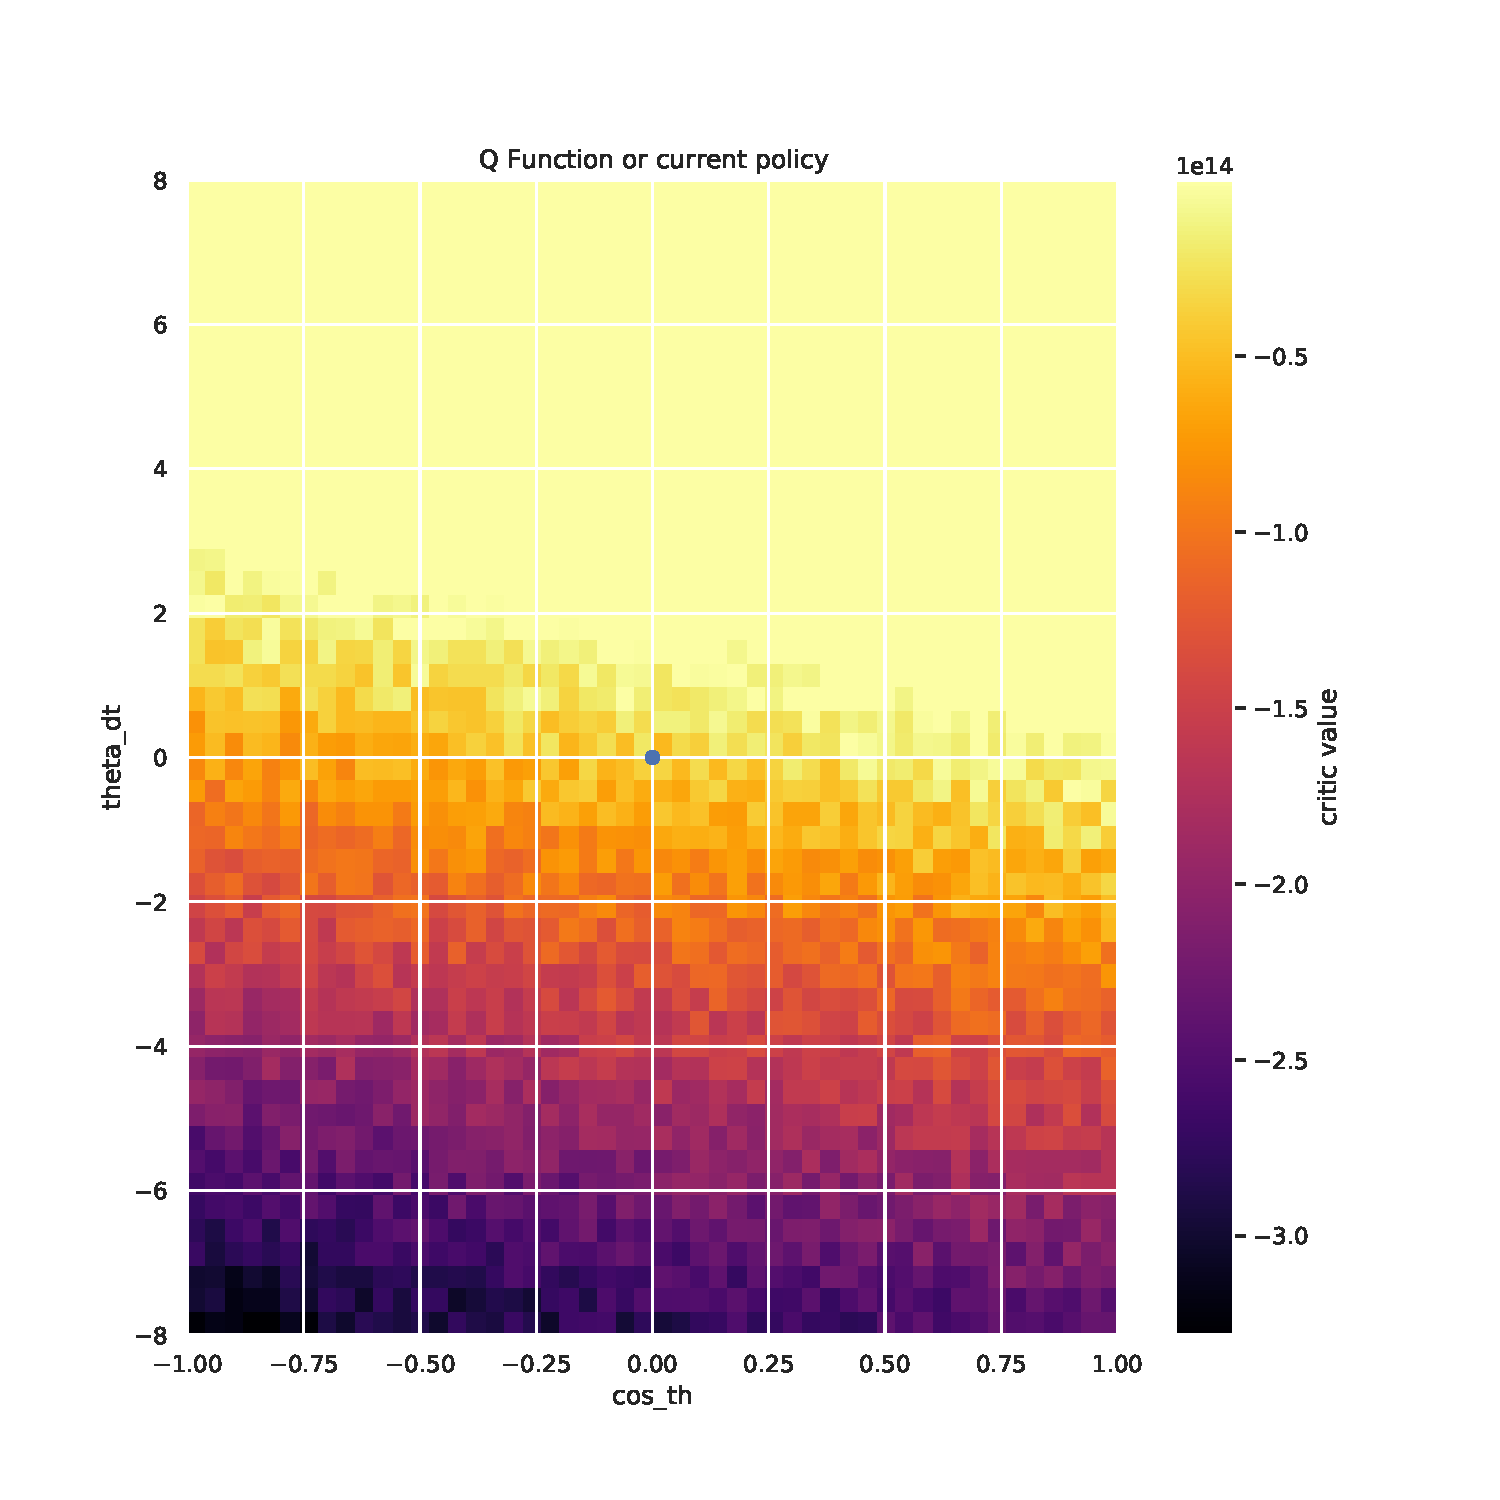
\includegraphics[width=\textwidth]{figures/iteration1/0_critic_discount_post_Pendulum-v0.pdf}
        \caption{Critique entraînée}
    \end{subfigure}
    \caption{Valeurs de l'acteur et de la critique avec la méthode discount pour le calcul de la récompense}
    \label{fig:attempt1_disount}
\end{figure}

Avec l'évaluation de l'acteur \emph{normal} dans la figure~\ref{fig:attempt1_disount}, la critique et l'acteur obtenus après entraînement sont quasi identiques. Mais les \emph{heatmaps} de ces derniers ne sont pas du tout satisfaisantes. En effet, la zone de préférence est située dans l'intervalle positif des vitesses angulaires. Or nous ne souhaitons absolument pas que l'IA favorise un mouvement mais une position d'équilibre en haut du pendule.

\begin{figure}[H]
    \centering
    \begin{subfigure}{0.3\textwidth}
        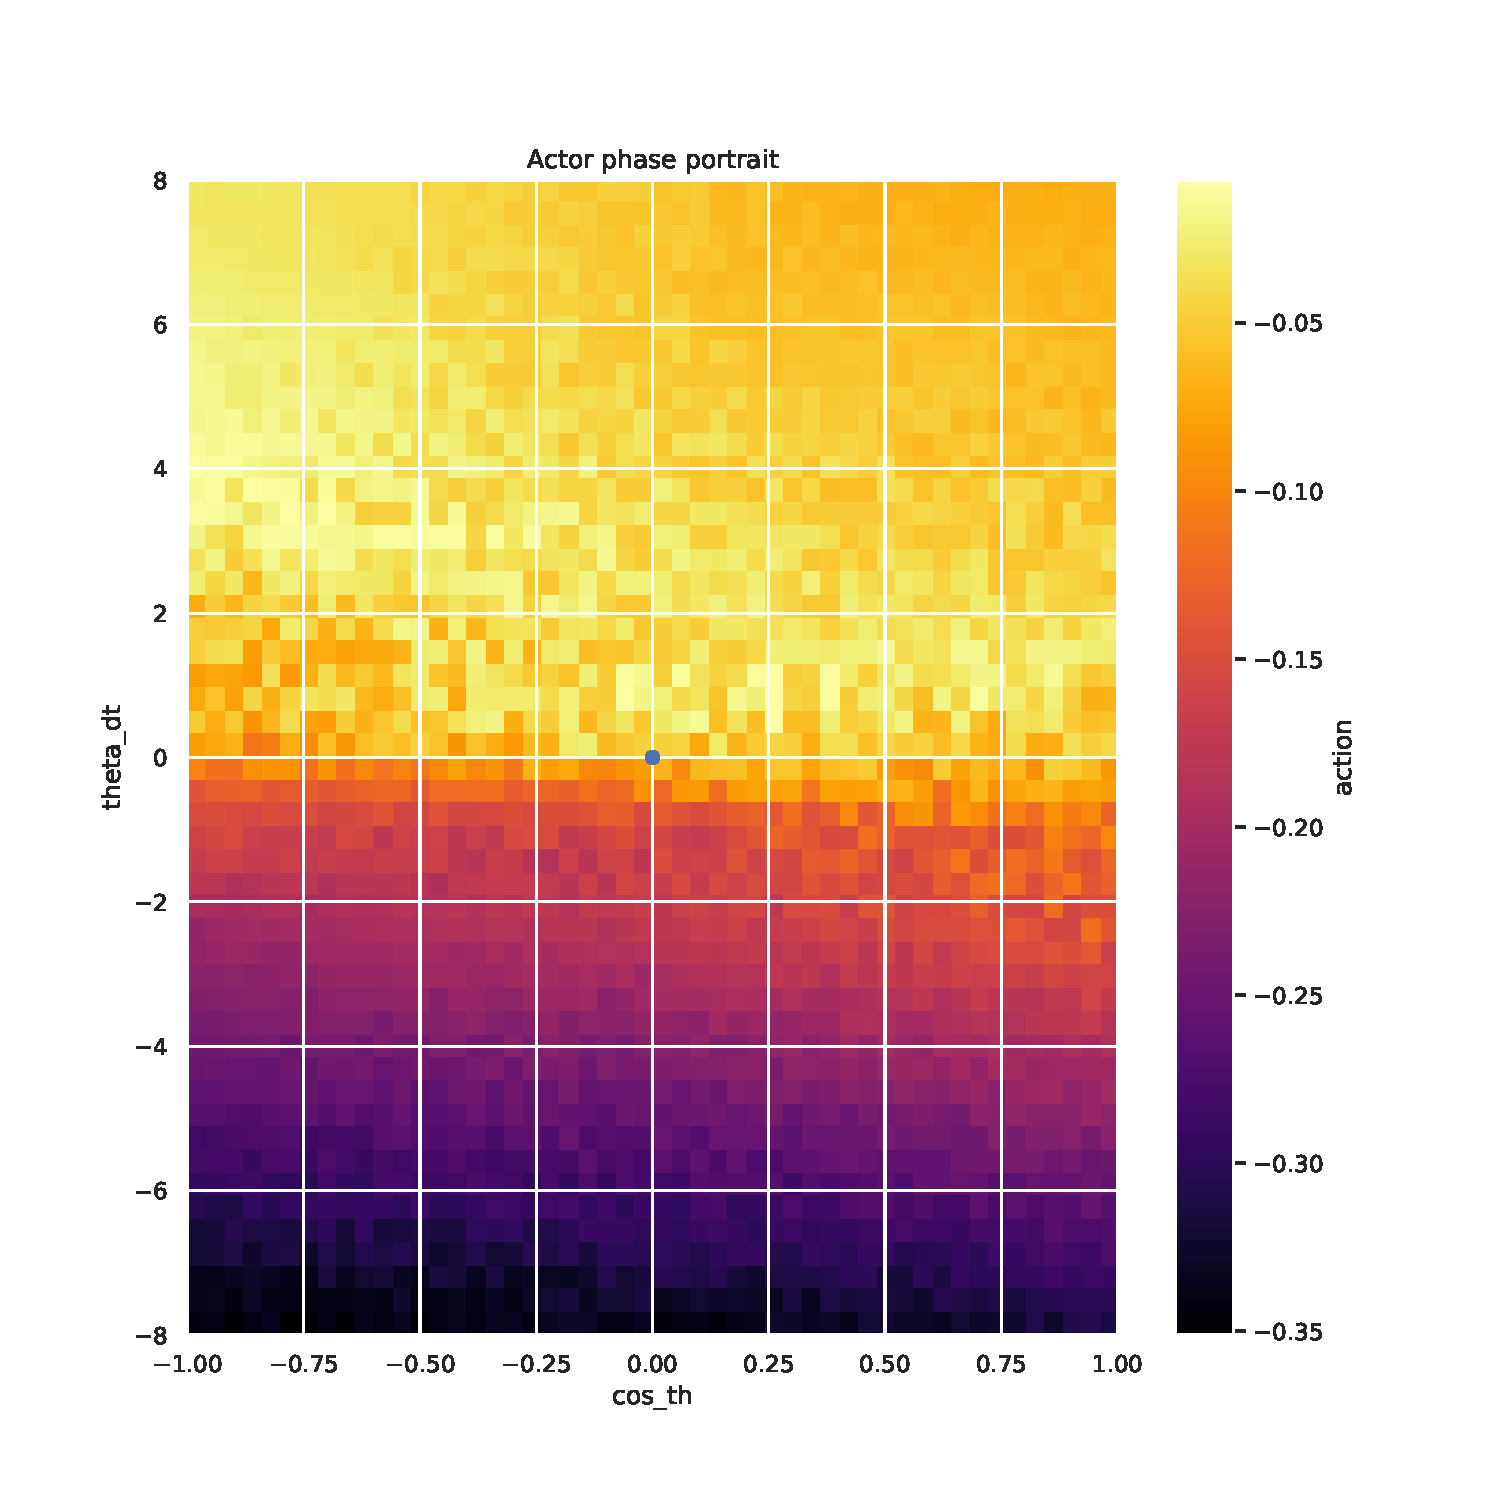
\includegraphics[width=\textwidth]{figures/iteration1/0_actor_normalize__ante_Pendulum-v0.pdf}
        \caption{Acteur naïf}
    \end{subfigure}
    \begin{subfigure}{0.3\textwidth}
        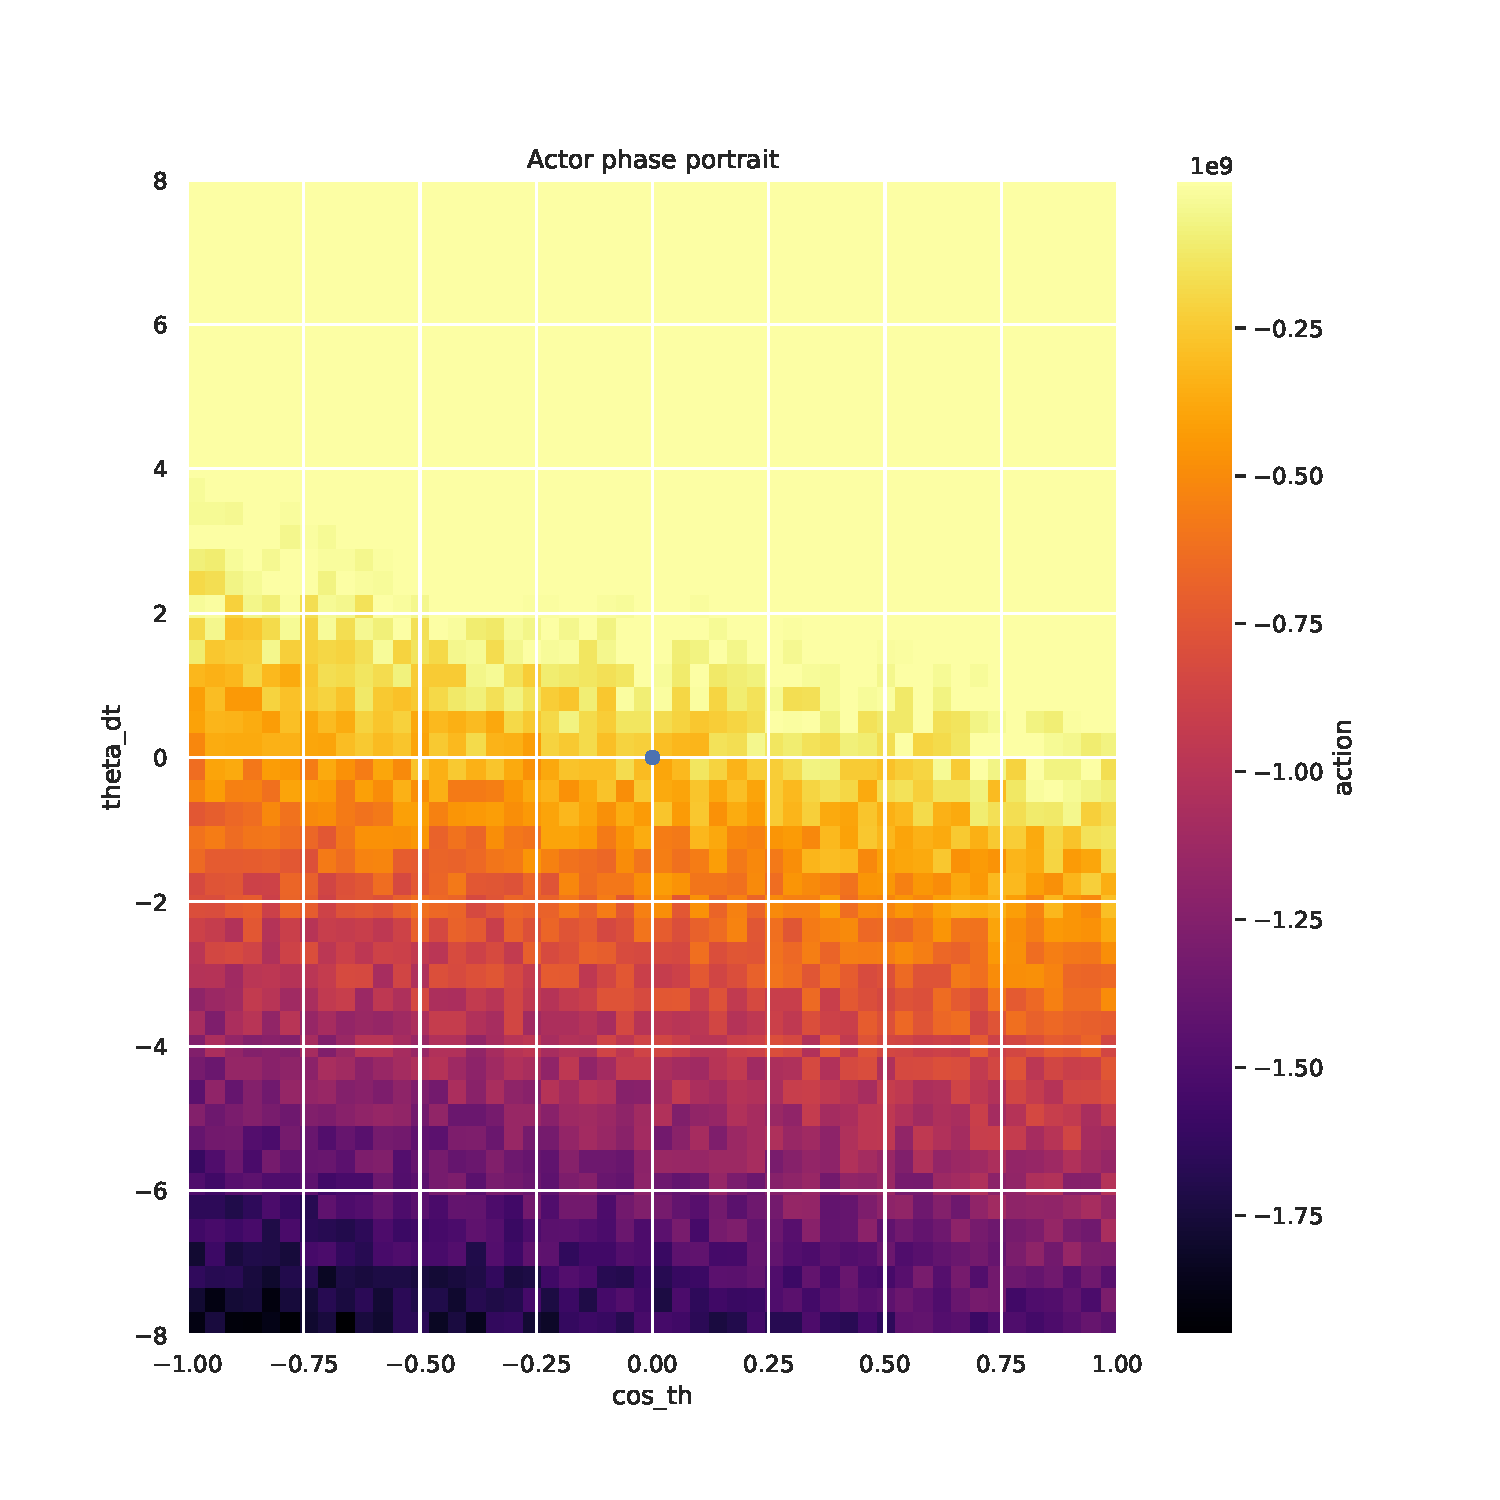
\includegraphics[width=\textwidth]{figures/iteration1/0_actor_normalize__post_Pendulum-v0.pdf}
        \caption{Acteur entraîné}
    \end{subfigure}
    \begin{subfigure}{0.3\textwidth}
        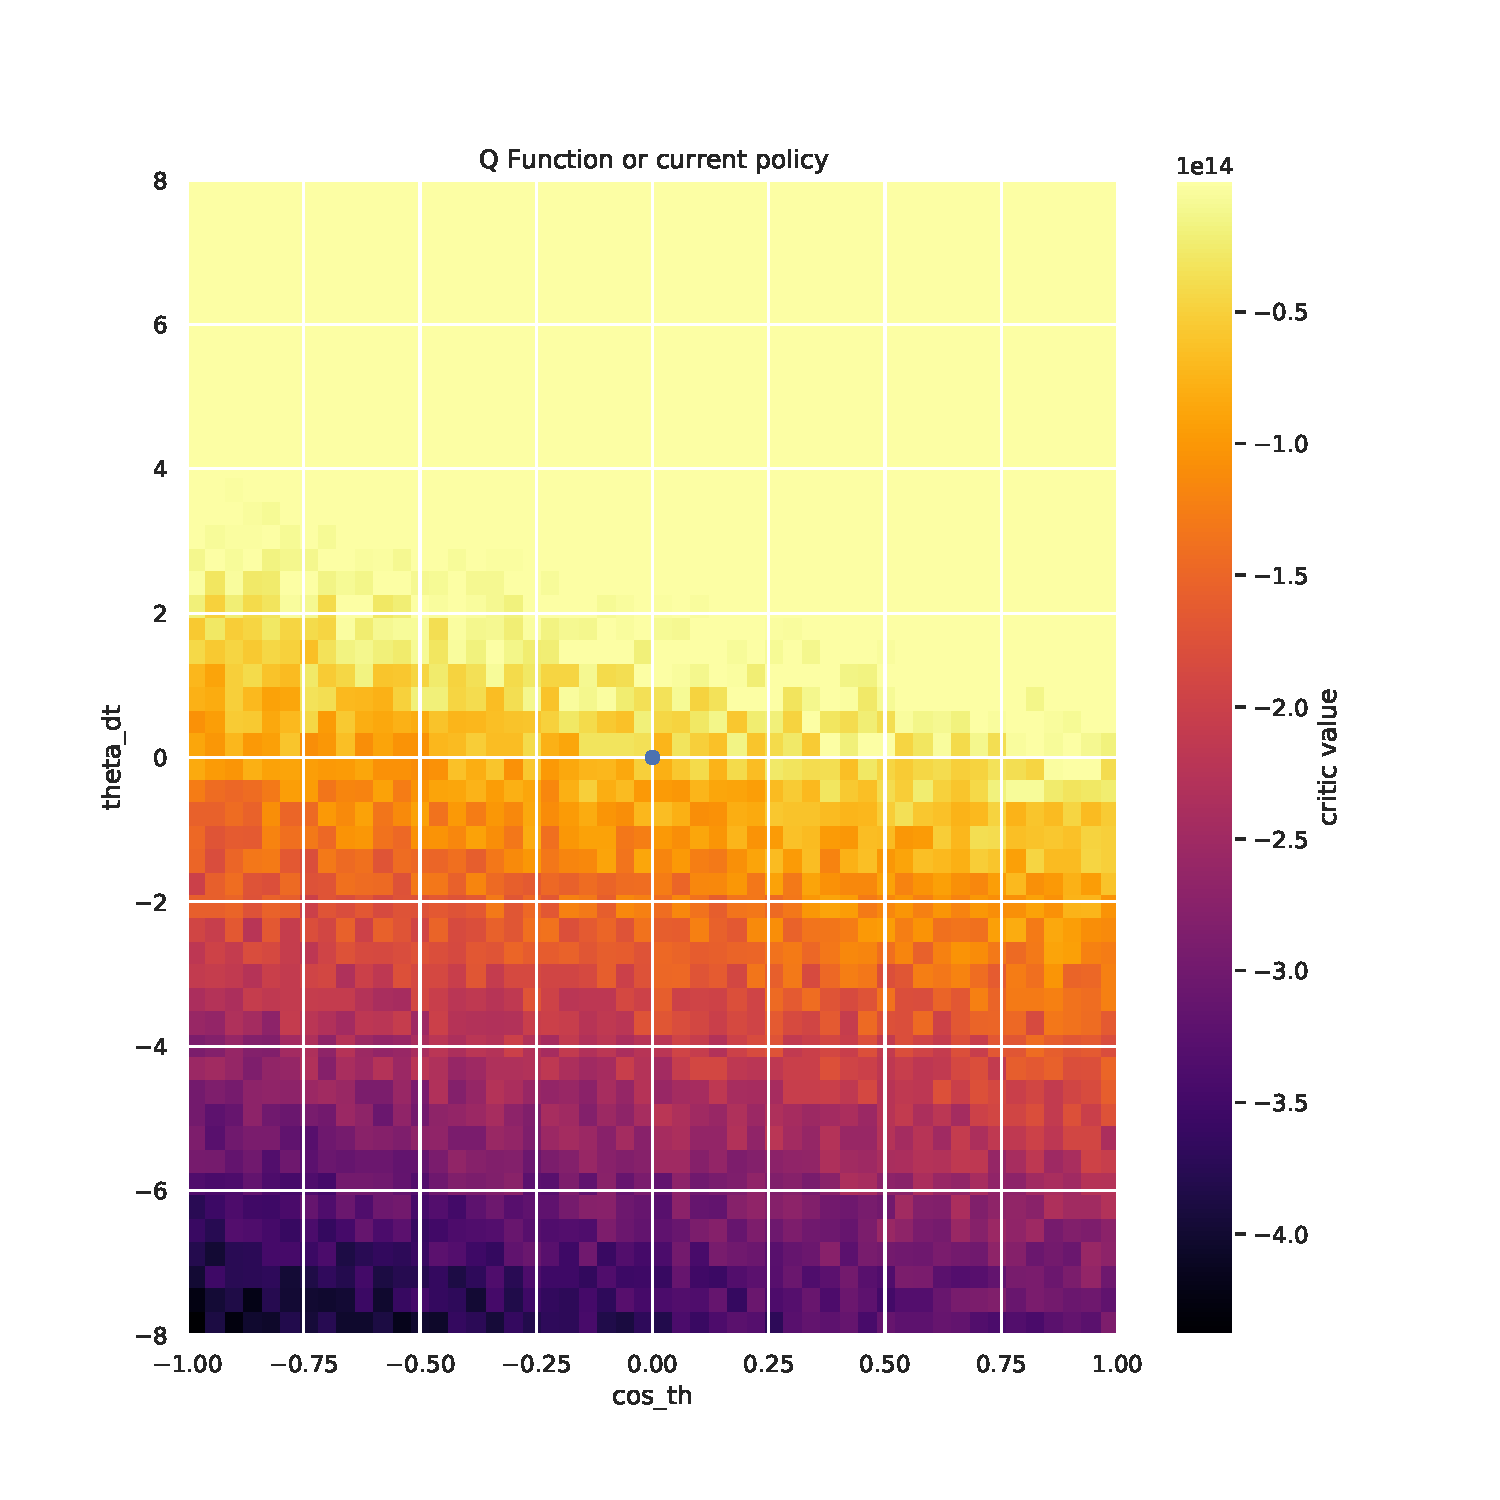
\includegraphics[width=\textwidth]{figures/iteration1/0_critic_normalize_post_Pendulum-v0.pdf}
        \caption{Critique entraînée}
    \end{subfigure}
    \caption{Valeurs de l'acteur et de la critique avec la méthode normale pour le calcul de la récompense}
    \label{fig:attempt1_normalize}
\end{figure}

Sur la figure~\ref{fig:attempt1_normalize} mis à part l'acteur naïf qui est différent parce qu'il est généré aléatoirement, l'acteur et la critique après entraînement sont identiques à ceux obtenus avec \emph{discount}. Ces résultats ne sont pas satisfaisant non plus.

\begin{figure}[H]
    \centering
    \begin{subfigure}{0.3\textwidth}
        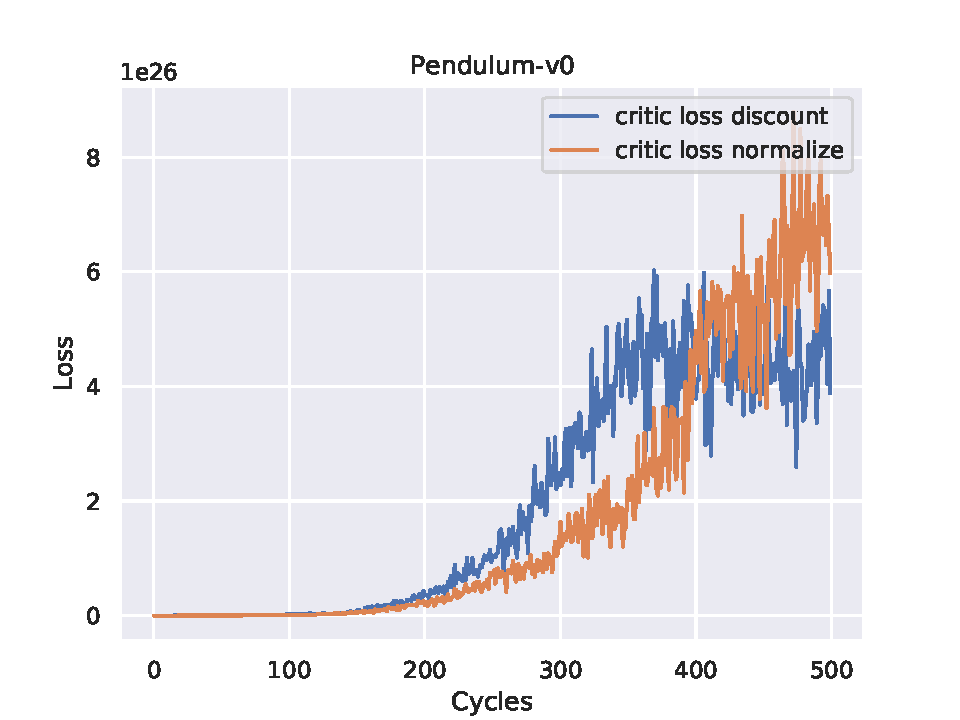
\includegraphics[width=\textwidth]{figures/iteration1/critic_loss_Pendulum-v0_pg_dataset_td_eval_True_cycles_500_trajs_20_batches_20_gamma_0.99_nstep_5_lr_act_0.01_lr_critic_0.01pg.pdf}
        \caption{Fonction de perte de la critique}
    \end{subfigure}
    \begin{subfigure}{0.3\textwidth}
        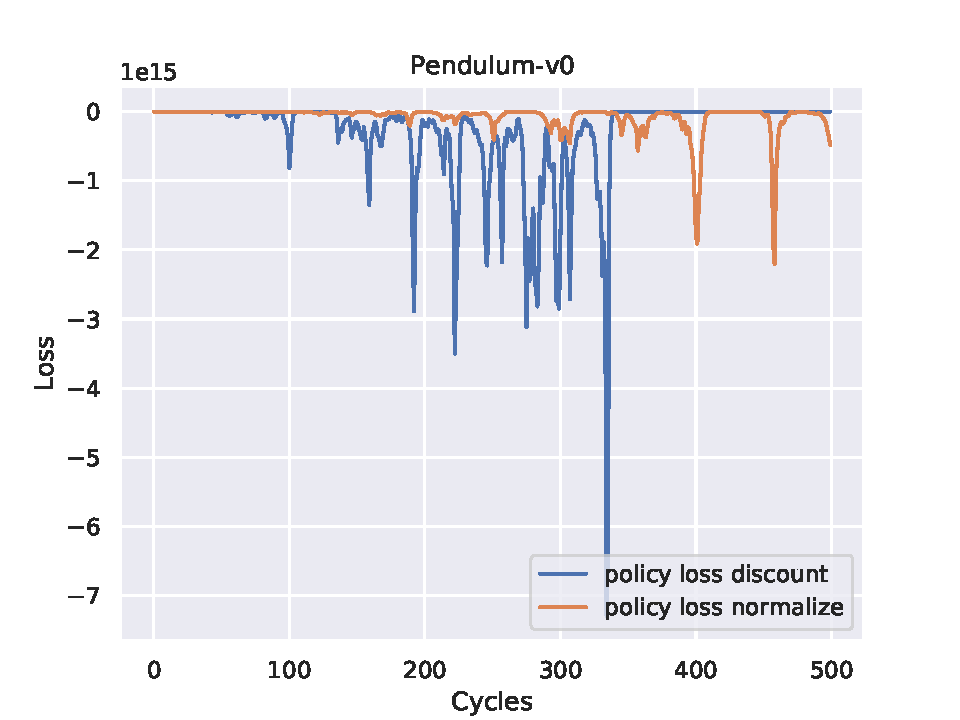
\includegraphics[width=\textwidth]{figures/iteration1/policy_loss_Pendulum-v0_pg_dataset_td_eval_True_cycles_500_trajs_20_batches_20_gamma_0.99_nstep_5_lr_act_0.01_lr_critic_0.01pg.pdf}
        \caption{Fonction de perte de la politique}
    \end{subfigure}
    \begin{subfigure}{0.3\textwidth}
        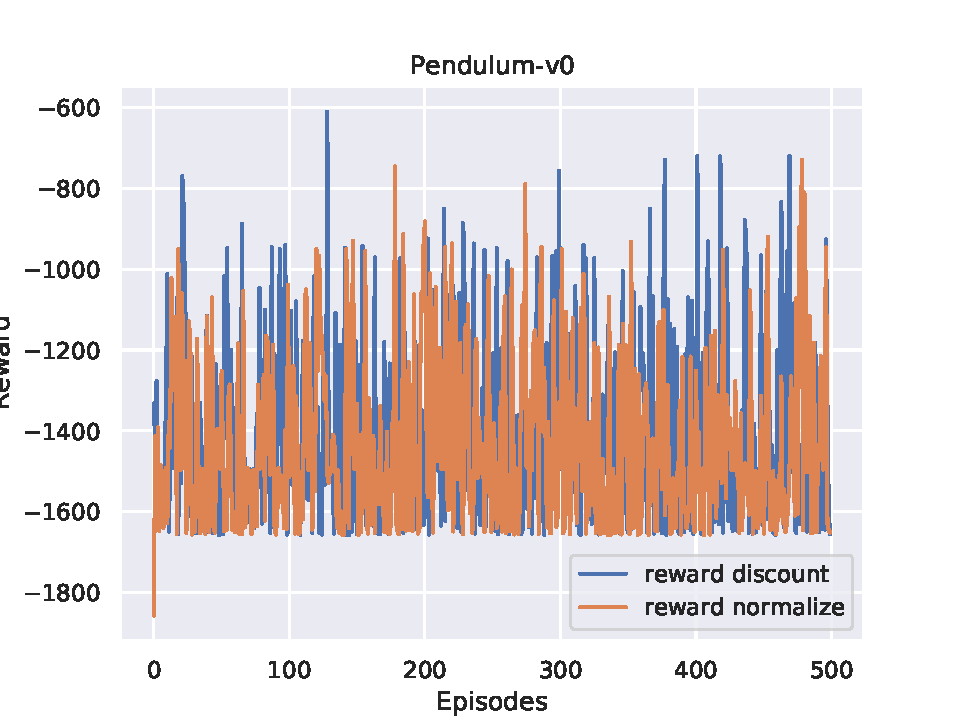
\includegraphics[width=\textwidth]{figures/iteration1/rewards_Pendulum-v0_pg_dataset_td_eval_True_cycles_500_trajs_20_batches_20_gamma_0.99_nstep_5_lr_act_0.01_lr_critic_0.01.pdf}
        \caption{Récompenses des épisodes}
    \end{subfigure}
    \caption{Résultats obtenus pour la critique, la politique et la récompense}
    \label{fig:attempt1_results}
\end{figure}

La figure~\ref{fig:attempt1_results} montre la perte de la méthode \emph{discount} se stabilise au bout de 350 cycles tandis que celle de la méthode \emph{normalize} continu de diverger. La fonction de perte de la critique est très mauvaise avec un ordre de grandeur de $1e15$ pour la perte. Mais on peut voir que la critique de la méthode \emph{normalize} est légèrement meilleur. Enfin la courbe des récompenses ne montre pas de convergence vers 0 que l'on attend. A contrario, il semble rester stagner au minimum, c'est à dire en bas du pendule, entre les épisodes.